% Ouverture sur une page
\documentclass[a4paper,11pt,oneside]{book} 

% +---------------------------------------------------------------+
% | Langue
% +---------------------------------------------------------------+
\usepackage[T1]{fontenc}
\usepackage[utf8]{inputenc}
\usepackage[american]{babel}


% +---------------------------------------------------------------+
% | Paramètres
% +---------------------------------------------------------------+

% confidentialité ? choisir la ligne non-commentée :
%\newif\ifisconfidential	\isconfidentialfalse % si NON confidentiel
\newif\ifisconfidential	\isconfidentialtrue % si confidentiel
\newcommand{\confidential}{\textbf{Confidential}} %Ce texte sera affiché dans chaque entête. 

% draft ? choisir la ligne non-commentée :
\newif\ifisdraft\isdraftfalse % si NON draft
%\newif\ifisdraft\isdrafttrue % si draft

% Font for HES-SO
\usepackage[scaled]{helvet}
\renewcommand*{\familydefault}{\sfdefault}

% Titles
\newcommand{\TMtype}{Master thesis}
\newcommand{\TMtitle}{Title example}
\newcommand{\TMsubtitle}{Subtitle}%laisser vide si pas de sous-titre
\newcommand{\TMyear}{2026}
\newcommand{\TMacademicYears}{2025-26}

% School
\newcommand{\TMfiliere}{Filière}
\newcommand{\TMfiliereData}{Master of Science HES-SO in Engineering}
\newcommand{\TMorient}{Profil}
\newcommand{\TMorientData}{Information and Cyber Security (ICS)}

% Student
\newcommand{\TMproducedby}{Produced by}
\newcommand{\TMauthor}{Author}
\newcommand{\TMauthorData}{First Last Name}

% Supervisor
\newcommand{\TMsupervisorData}{Prof. First Last Name}
\newcommand{\TMsupervisor}{Under the supervision of \TMsupervisorData}

% Industry
\newcommand{\TMindustryType}{Industrial partner}
\newcommand{\TMindustryName}{IndustryName}
\newcommand{\TMindustryContact}{First Last Name}
\newcommand{\TMindustryAddress}{%
  Rue XY\\
  1234 Ville
}
\newcommand{\TMindustry}{In collaboration with \TMindustryName}

% Date and location
\newcommand{\Date}{Date of publication}
\newcommand{\DateData}{\today}
\newcommand{\LieuSignature}{Yverdon-les-bains}

% Footer
\newcommand{\FooterTL}{Master of Science in Engineering (MSE)}
\newcommand{\FooterBL}{Master thesis}
\newcommand{\FooterTM}{\TMauthorData}
\newcommand{\FooterBM}{%
	\ifisconfidential
		\textcolor{red}{Confidential}
	\else
		Non-confidential
	\fi
	}
\newcommand{\FooterTR}{\DateData}



\newcommand{\TMresumePubliable}{
	\lipsum[6] % exemple

	Ceci est le résumé publiable...

	Rappel du contexte et de la problématique

	Dans ce travail, il a été réalisé

	Présenter les résultats et ce que cela a apporté	
	
	\lipsum[2] % exemple
}

% +---------------------------------------------------------------+



% +-[set path]-------------------------------------+
\usepackage{template/TM-style}
\usepackage{template/TM-macros}
\usepackage{template/TM-template}
%\graphicspath{images/}
\usepackage{hyperref} %Doit etre le dernier package


\begin{document}

\frontmatter

% TITLE 
% +---------------------------------------------------------------+
\pagestyle{empty}
\TMmaketitle

% template parts
% +---------------------------------------------------------------+
\pagestyle{mainstyle}

% TOC ----------------------------------------------------------+
\tableofcontents
\clearpage

\chapter{Declaration of authenticity}
I hereby affirm that this assignment is my own written work and that I have used no other sources or aids other than those indicated. All passages that have been quoted from publications or paraphrased from these sources are indicated as such. Additionally, any assistance from artificial intelligence tools has been appropriately acknowledged and documented.
\vspace{1cm}

\begin{flushright}
    \begin{minipage}{7cm}
        Date : {\DateData}
        Name : {\TMauthorData}
    \end{minipage}
\end{flushright}


\chapter{Acknowledgments}
To write...


\chapter{Summary}
To write (in English)...


\chapter{Résumé}
A écrire (en français)...


% Content
% +---------------------------------------------------------------+
\mainmatter
\fullchaptermarktrue %affiche les chapitres complets, exemple : Chapitre N : Titre

\input{chapters/introduction}

% +---------------------------------------------------------------+
% indique quel est le document Master à compiler
% TeXstudio
% !TeX master = ../tb_report.tex
%
% TexShop
% !TEX root = ../tb_report.tex

\chapter{Specification}


\section*{Problem statement}
\lipsum[110-111]

\section*{Objectives}
\todo{Redefine it}
\lipsum[1-1]

\subsection*{Timeline}
The work begins on … and ends on …. During the first 16 weeks, from x to y, the workload is 12 hours per week. During the final 6 weeks, from x to y, this work will be carried out full-time.

A graded interim submission is required on x, and the final submission is scheduled for x at 12:00.

The defense will take place between x and y.

\subsection*{Tasks}
%exemple
\lipsum[1-1]

\subsection*{Deliverables}
\todo{to check}
The deliverables will be as follows:
\begin{enumerate}
	\item A documentation including:
	      \begin{itemize}
		      \item A market analysis
		      \item The decision resulting from this analysis
		      \item Specifications
		      \item Information about the module, such as its operation and limitations
		      \item An initial and a final project plan
		      \item A user manual
	      \end{itemize}
	\item A module fulfilling the objectives defined in Section 2.1.
	\item Software implementing the improvements, if it has been possible to carry them out.
\end{enumerate}


\input{chapters/planification}

% +---------------------------------------------------------------+
% indique quel est le document Master à compiler
% TeXstudio
% !TeX master = ../tb_report.tex
%
% TexShop
% !TEX root = ../tb_report.tex

\chapter{State of the art}
\label{ch:stateoftheart}


%exemple
\lipsum[1-4]



% +---------------------------------------------------------------+
% Indicates which master document to compile
% TeXstudio
% !TeX master = ../tb_report.tex
%
% TeXShop
% !TEX root = ../tb_report.tex

\chapter{Example of Chapter}

\lipsum[1]


\section{Writing Mathematical Expressions}
\todo{example of todo}

Here is an inline math example: $3^2 / 4^3$.

Or on a separate line:

$$ \frac{3 x_a}{ y_b^2 +4}$$

\section{Inserting Images}

Here is how to insert an image.

\begin{figure}
	\centering
	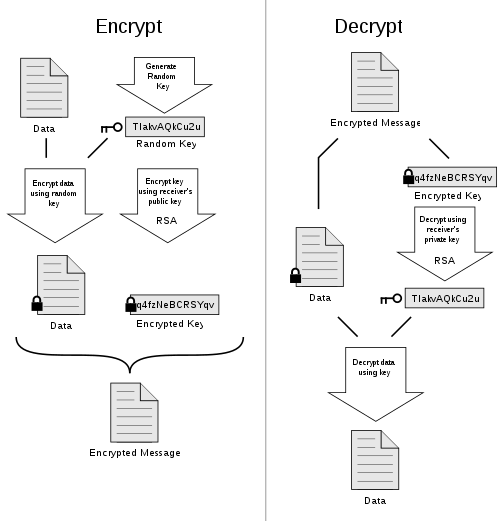
\includegraphics[width=8cm]{images/PGP_101.png}
	\caption{PGP Diagram}
	\label{fig:pgp}
\end{figure}


\section{Creating and Citing Bibliographic References}
\todo{improve my bibliography}

This is an example of citing a book by Pasini~\cite{pasini2015}.

But also a website, Black Alps 2019~\cite{BA19}!


\section{Creating References to Other Parts of the Document}

You can also add a reference to Section~\ref{sec:shell}.

You can also add a reference to the introduction, Chapter~\ref{ch:intro}.

As shown in Figure~\ref{fig:pgp}, you can reference a figure.


\section{Displaying a Simple Command or Bash}

Use the command \com{com}.

Example: Testing a bash shell command \com{ls}:

Use the environment \com{shellcmd}.

\begin{shellcmd}
	$> ls -al test_underscore $$* "hello"
\end{shellcmd}
Blah blah


\section{Displaying a Shell Command}
\label{sec:shell}

Here is how to format a SHELL command.

Use the \com{listingsbox} environment.
\begin{description}
	\item[1st parameter:] the type of shell, here "console"
	\item[2nd parameter:] the name to give to the box
\end{description}

\begin{listingsbox}{console}{Example of shell command with output}
	root@kali:~$ bunzip2 data-decrypted.bin
	bunzip2: Can't guess original name for data-decrypted.bin -- using
	data-decrypted.bin.out
\end{listingsbox}


\section{Including Code in LaTeX}

Use the \com{sourcebox} environment.
\begin{description}
	\item[1st parameter:] the language, here "c"
	\item[2nd parameter:] the name to give to the box
\end{description}

\begin{sourcebox}{c}{Example C code}
	#include <stdio.h>

	int main(int argc, char* argv[])
	{
			printf("Hello World!\n");
			return 0;
	}
\end{sourcebox}



\section{Including Code from an External Source File}

Use the command \com{inputsourcecode}.
\begin{description}
	\item[1st parameter:] the language, here "c"
	\item[2nd parameter:] the source file name, "\path{source_code/example.c}"\\ Also an example of the \com{path} command.
	\item[3rd parameter:] the name to give to the box
\end{description}


%% Include source code from an external file
%% 1st parameter: code language
%% 2nd parameter: path to the source file
%% 3rd parameter: title of the box
\inputsourcecode{c}{source_code/example.c}{example.c}

Same example, but specifying lines 4 to 8:
\inputsourcecode[firstline=4,lastline=8]{c}{source_code/example.c}{example.c}

\input{chapters/architecture}

\input{chapters/implementation}

% +---------------------------------------------------------------+
% indique quel est le document Master à compiler
% TeXstudio
% !TeX master = ../tb_report.tex
%
% TexShop
% !TEX root = ../tb_report.tex

\chapter{Results}
\label{ch:results}


%exemple
\lipsum[1-4]


\input{chapters/conclusion}


% +---------------------------------------------------------------+
\cleardoublepage
\phantomsection
\addcontentsline{toc}{chapter}{Bibliography}
\markboth{Bibliographie}{Bibliography}
%\bibliographystyle{plain}
\bibliographystyle{alpha}
\bibliography{chapters/biblio}
\nocite{*} %ajoute tout ce qu'il y a dans le bibtex

\phantomsection
\listoffigures
\addcontentsline{toc}{chapter}{List of Figures}
\markboth{Table des Figures}{List of Figures}

\phantomsection
\listoftables
\addcontentsline{toc}{chapter}{List of Tables}
\markboth{Liste des tableaux}{List of Tables}


% Annexes
% +---------------------------------------------------------------+
\appendix

% +---------------------------------------------------------------+
% indique quel est le document Master à compiler
% TeXstudio
% !TeX master = ../tb_report.tex
%
% TexShop
% !TEX root = ../tb_report.tex

\chapter{Tools used for environment tests}

%exemple
\lipsum[5-6]


% +---------------------------------------------------------------+
% Indicates which master document to compile
% TeXstudio
% !TeX master = ../tb_report.tex
%
% TeXShop
% !TEX root = ../tb_report.tex

\chapter{Log Book}

\begin{landscape}

	\begin{longtable}[c]{lp{10cm}rrrr}
		\caption{Work Journal}                                                                                               \\

		\hline
		Date & Description                                                        & Research [h] & Dev. [h] & Report [h] & Admin [h] \\
		\hline
		\endfirsthead

		\hline
		Date & Description                                                        & Research [h] & Dev. [h] & Report [h] & Admin [h] \\
		\hline
		\endhead

		\multicolumn{6}{r}{\small \it The log book continues on the next page.}                                          \\
		\normalsize
		\endfoot

		\hline
		\endlastfoot


		% Work
		5.03.2026
		     & Kick-off meeting with the client \lipsum[1-1]
		     & 0                                                                                                                   %research
		     & 0                                                                                                                   %dev
		     & 0                                                                                                                   %report
		     & 2                                                                                                                   \\ %admin

		12.03.2026
		     & Research on the state of the art
		     & 4                                                                                                                   %research
		     & 0                                                                                                                   %dev
		     & 0                                                                                                                   %report
		     & 0                                                                                                                   \\ %admin

		19.03.2026
		     & Setup of the development environment and documentation
		     & 0                                                                                                                   %research
		     & 7                                                                                                                   %dev
		     & 1                                                                                                                   %report
		     & 0                                                                                                                   \\ %admin

		25.03.2026
		     & Writing the state-of-the-art section
		     & 0                                                                                                                   %research
		     & 0                                                                                                                   %dev
		     & 4                                                                                                                   %report
		     & 0                                                                                                                   \\ %admin

		25.03.2026
		     & Development of the interface part
		     & 0                                                                                                                   %research
		     & 0                                                                                                                   %dev
		     & 4                                                                                                                   %report
		     & 0                                                                                                                   \\ %admin


		xx.xx.2026
		     & Testing
		     & 0                                                                                                                   %research
		     & 0                                                                                                                   %dev
		     & 4                                                                                                                   %report
		     & 0                                                                                                                   \\ %admin

		xx.xx.2026
		     & Testing
		     & 0                                                                                                                   %research
		     & 0                                                                                                                   %dev
		     & 4                                                                                                                   %report
		     & 0                                                                                                                   \\ %admin

		xx.xx.2026
		     & Testing
		     & 0                                                                                                                   %research
		     & 0                                                                                                                   %dev
		     & 4                                                                                                                   %report
		     & 0                                                                                                                   \\ %admin

		xx.xx.2026
		     & Testing
		     & 0                                                                                                                   %research
		     & 0                                                                                                                   %dev
		     & 4                                                                                                                   %report
		     & 0                                                                                                                   \\ %admin

		xx.xx.2026
		     & Testing
		     & 0                                                                                                                   %research
		     & 0                                                                                                                   %dev
		     & 4                                                                                                                   %report
		     & 0                                                                                                                   \\ %admin

		xx.xx.2026
		     & Testing
		     & 0                                                                                                                   %research
		     & 0                                                                                                                   %dev
		     & 4                                                                                                                   %report
		     & 0                                                                                                                   \\ %admin

		xx.xx.2026
		     & Testing
		     & 0                                                                                                                   %research
		     & 0                                                                                                                   %dev
		     & 4                                                                                                                   %report
		     & 0                                                                                                                   \\ %admin

		xx.xx.2026
		     & Testing
		     & 0                                                                                                                   %research
		     & 0                                                                                                                   %dev
		     & 4                                                                                                                   %report
		     & 0                                                                                                                   \\ %admin

		xx.xx.2026
		     & Testing
		     & 0                                                                                                                   %research
		     & 0                                                                                                                   %dev
		     & 4                                                                                                                   %report
		     & 0                                                                                                                   \\ %admin

		xx.xx.2026
		     & Testing
		     & 0                                                                                                                   %research
		     & 0                                                                                                                   %dev
		     & 4                                                                                                                   %report
		     & 0                                                                                                                   \\ %admin
	\end{longtable}

\end{landscape}


\end{document}
